\documentclass[sigconf]{acmart}
%%
%% \BibTeX command to typeset BibTeX logo in the docs
\AtBeginDocument{%
  \providecommand\BibTeX{{%
    \normalfont B\kern-0.5em{\scshape i\kern-0.25em b}\kern-0.8em\TeX}}}


\newcommand\myworries[1]{\textcolor{red}{#1}}

%%%%%%%%%%%%%%%%%%%%%%%%%%%%%%%%%%%%%%%%
% Inverting Colors to save my eye balls
%\usepackage{xcolor}
%\pagecolor[rgb]{0.1,0.12,0.15}
%\color[rgb]{.9,.9,.95}
%%%%%%%%%%%%%%%%%%%%%%%%%%%%%%%%%%%%%%%%

\citestyle{acmauthoryear}



\begin{document}

\title{The Shape Matching Element Method for Meshless Animation of NURBs Models}

%% A "teaser" image appears between the author and affiliation
%% information and the body of the document, and typically spans the
%% page.
\begin{teaserfigure}
  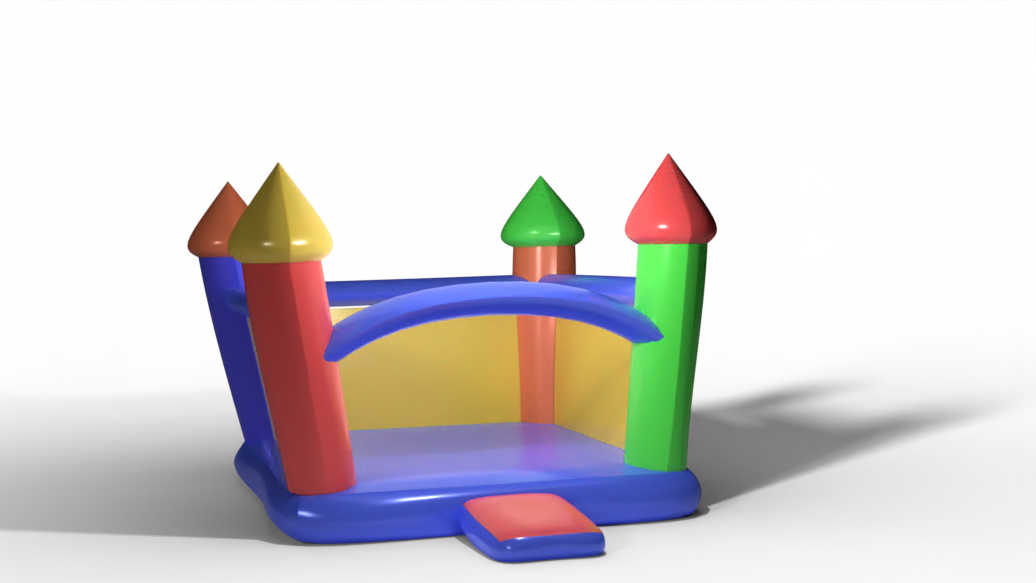
\includegraphics[width=\textwidth]{castle.png}
  \caption{tmp}
  \Description{}
  \label{fig:teaser}
\end{teaserfigure}

\maketitle

\section{Introduction}

The consumption of geometric surface models by physics-based animation algorithms is fraught with difficulty. 
For volumetric objects, this process often involves identifying and discretizing the interior of the modelled object, 
typically either as a tetrahedral or hexahedral mesh.%
This procedure is both expensive and difficult, especially if the surface model is constructed from higher-order boundary
representations, or if the volumetric discretization is required to be conforming or feature aligned. 
Removing explicit volumetric discretization from the physics-based-animation pipeline can avoid these difficulties and 
also provide a more unified modelling and simulation experience. 

NURBS (Non-uniform Rational B Splines) are a popular higher-order modelling primitive which 
are used for computer-aided design (CAD), computational fabrication and computer animation. 
NURBS primitives were the first geometric representation used for physics-based animation, yet,
despite over three decades of research, animation of NURBS objects remains a challenge.

Isogeometric Analysis (IGA) is a physics simulation methodology that uses the control variables of the NURBS model
as the degrees-of-freedom (DOFS) of the simulation itself. 
Unfortunately IGA approaches for volumetric objects still require background volumetric structures, typically
regular grids that make satisfaction of boundary conditions difficult (which makes collision resolution difficult)
or more complicated cut-cell grids which introduce non-trivial root finding problems into the mix. 
Crucially, these simulation schemes typically assume models arise from engineering applications and meet tight geometric
criteria such as that the mesh is manufacturable. 
These inputs are much cleaner than those produced by a typical modeller. 

% In this paper we present a new finite element method for isogeometric, physics-based animation of NURBs models.
% Crucially our method is boundary only, and requires no volumetric meshes (thus avoiding their inherent complications), grids or cutcells of any kind
% Our method does not need an explicit labelling of the inside/outide of the simulated model
% Does not require nurbs patches in an object to be explicitly joined
% Input is just the raw NURBs model with no additional information or annotations
% The resulting simulation algorithm is compatiable with nonlinear continuum mechanics material models as well as 
% standard methods for contact resolution. 

We present the first truly meshless (no volumetric discretization generated) algorithm for direct, nonlinear elastodynamic simulation of NURBs models. 
Our nonlinear elastodynamic simulation scheme requires only a boundary description of the object (we do not strictly require a solid model) and
approriate physical parameters.  
Because we explicitly use the NURBS boundary representation in the simulation its is straightforward to handle
Dirichilet, Neumann boundary conditions and to apply contact resolution. 
Crucially because we broadly target animation not necessarily simulation for engineering or manufacturing we don't require that models
satisfy the rigourous geometric requirements common for these applications

Our approach is an extension of the recently developed Virtual Element Method (VEM) for solving PDEs on domains tiled with arbitrary polygons.
We establish a connection between VEM and the well-known shape matching simulation algorithm  which enables us 
to derive equations of motion for an arbitrary NURBS model using Lagrangian Mechanics. 
Importantly, we show how to replace volumetric data structures for integration with ray casting approaches which enables
our meshless approach to isogeometric elastodynamic simulation of volumetric structures.

% Modelling -> Animation -> Rendering
% Use physics for animation which requires conversion from modelling to simulation representation
% for volumetric objects this conversion invovles identififyin and meshing the interior of the modelled object and that's hard
% especially difficult if object surface is described by higher-order boundary representations. 
% Ideally we would have a more direct method of translating our surface model into a volumetric, simulatable form
%
% NURBs  are an oft-used higher order modelling primitive popular for CAD and Computer Graphics for which nice modelling tools exist
% Rhinocerous 3D and Fusion 360.
% Despite lots of work performing physics-based animation on NURBS models is hard
% robustly uilding a volumetric polygonal mesh that simulataneously maintains a corresonpondence to the model surface is an open-research problem
% Isogeometric approaches which directly use the NURBs primitives as simulation variables require additional background grids, complex cutcell algorithms
% and often must rely on soft boundary conditions.
%
% Want to say there is an advantage to avoiding constructing volumetric representations because it costs time and adds complexity
% that;s our goal to provide an alternative, the first truly meshless approach to IGA which maintains a tightt mapping to the boundary
% In this paper we present a new finite element method for isogeometric, physics-based animation of NURBs models.
% Crucially our method is boundary only, and requires no volumetric meshes (thus avoiding their inherent complications), grids or cutcells of any kind
% Our method does not need an explicit labelling of the inside/outide of the simulated model
% Does not require nurbs patches in an object to be explicitly joined
% Input is just the raw NURBs model with no additional information or annotations
% The resulting simulation algorithm is compatiable with nonlinear continuum mechanics material models as well as 
% standard methods for contact resolution. 
%
% crucially because we broadly target animation not necessarily simulation for engineering or manufacturing we don't require that models
% satisfy rigourous geometric requirements common for these applications
%
% Our approach relies on the recently developed Virtual Element Method for solving PDEs on domains tiled with arbitrary polygons.
% By establsihing the connection between VEM and the well-known shape matching simulation algorithm we derive equations of motion sfor 
% an arbitrary NURBS model using Lagrangian Mechanics. We avoid using volumetric data structures for integration by demonstrating that 
% raycasting provides a fast and reliable alternative. In combination, our contributions amount to the first algorithm for 
% isogeometric elastodynamics of volumetric structures that is truly meshless (introducing no auxilillary volumetric data structures) 
% which serves to close the considerable gap betweeen modelling and physics-based animation. 
%
% Desiderata for a sucessful algorithm for PBA 
% No volumetric mesh creation
% Support for Nonlinear Constitutive Models
% Support for standard Collision 
% DOFS on the Boundary (useful for boundary conditions, contact)
% Automatic determination of model volume
% Non-manufacturable models 
% Code Available 

%limitations
% sometimes you want some volumetric dofs to better resolve internal behaviour
\section{Related Work}

%% Set the scene
Geometric modeling is a necessary precursor to physics-based animation, however connecting differing geometric representations for modelling and simulation often requires
time-consuming, complex geometry processing pipelines. 
For instance, the popular tetrahedral finite element approach for simulating solid elastodynamics~\cite{10.1145/2343483.2343501} requires robust algorithms for converting input surface geometry into 
a volumetric tetrahedral mesh. This is a difficult problem and while significant progress has been made,
even the most robust volumetric methods~\cite{Hu:2018:TMW:3197517.3201353} can be time consuming, fail to maintain correspondence between the input model and output simulation mesh,
and don't work directly on curved surface representations such as NURBS.  

%% Outline desiderata for success
%- no meshing of any kind, no tet, hex cut cells, nothing
%- simulation can be directly imported and edited in modelling software
%- supports standard continuum mechanics constitutive models
%- supports different time integrators (can show a few maybe linearly implicit, fully implicit and RK4 ?)

For many physics-based animation tasks, it would be desirable to bypass volumetric meshing entirely and directly simulate the geometric model.
An ideal approach would avoid meshing of any kind (no volumetric meshes or cut-cells), support continuum mechanics-type constitutive models 
and energies that have become standard in physics-based animation pipelines, be compatible with a wide range of time integration schemes and
ensure that simulation output can be edited in the same modelling software used to create the input (important for post-processing). 
Finally, our method should put only moderate constraints on input model quality to facilitate ease-of-use.

\emph{Isogeometric Analysis}~\cite{10.1002/9780470749081.ch7} endeavors to perform simulation directly on the NURBS output from 
Computer-Aided Design (CAD) software. Initial attempts used NURBS surfaces to represent the medial surface of thin objects~\cite{10.1145/176579.176580}.
Volumetric simulations relied on volumetric NURBS~\cite{10.1007/978-3-642-03596-8_2} but were limited to a narrow class of geometries.
Finite volume methods are applicable to more general geometries~\cite{HEINRICH20121645,10.1002/nme.2311} but require a volumetric mesh to be generated.
Modern approaches are constructed around the extended finite element method which enriches the standard finite element basis with discontinuous basis functions
to improve boundary handling~\cite{https://doi.org/10.1002/nme.3120,10.1007/s00466-013-0854-7,https://doi.org/10.1002/nme.4852,SAFDARI2016373,10.1145/3355089.3356576}. 
These methods typically start with an easy-to-generate structured volumetric mesh (tetrahedral or hexahedral), ``cutting'' the NURBS geometric model against
it to enable boundary handling (such a mesh is called a \emph{cut-cell} mesh). 
Like volumetric meshing, this cutting operation can be difficult and our ideal method would avoid it. 
Some cut-cell algorithms assume engineering/manufacturing quality input, which puts tight requirements on input models~\cite{10.1145/3355089.3356576}.
Finally these approaches require additional mechanisms to ensure that simulation results lie inside the shape space of the input model's primitives,
which increases the complexity. 

\revise{
\emph{Embedded Methods} attempt to sidestep many of these issues by enclosing complex surface geometry inside a simulation coarse mesh~\cite{10.5555/1009379.1009573}. 
However, producing an appropriate mesh embedding introduces a number of challenges since the coarse mesh's connectivity must mirror that of the embedded surface.
This necessitates the use of complex hierarchical methods like that of~\citet{10.1145/1531326.1531358}, which themselves require the user to correctly intuit an appropriate ultimate grid resolution.
Alternately one can introduce cut cell~\cite{Tao:Mandoline:2019} or extended Finite Element~\cite{10.1145/3355089.3356576} approaches which bring with them complicated geometric operations. 
Furthermore when the DOFs do not lie on the boundary, methods such as Nitsche's Method ~\cite{Nitsche1971berEV} are required for handling Dirichlet boundary conditions. 
Our method inherits shape connectivity directly from the boundary input, avoiding these difficulties entirely.
}

\emph{Shape Matching} is a meshless approach to physics-based animation~\cite{10.1145/1073204.1073216,10.1145/2019406.2019438} and geometry processing~\cite{10.1111/j.1467-8659.2012.03171.x}
built around shape registration. The algorithm has been extended from volumetric triangle mesh input to cloth~\cite{10.2312/PE/vriphys/vriphys08/039-046}, to particles~\cite{10.1145/1964921.1964987}
and even to visual geometry for video games~\cite{10.1145/2994258.2994260}. 
Shape Matching is fast~\cite{10.1145/1275808.1276480,10.5555/1632592.1632606} and meshless, but state-of-the-art methods require 
additional modelling input to position simulation primitives~\cite{10.1145/1964921.1964987} or limit simulation primitives to be 
collections of convex polytopes~\cite{10.1145/2994258.2994260}.
Finally, Shape Matching is tightly coupled to the position-based dynamics (PBD)~\cite{muller2007position}
time integration methodology. 
While incredibly performant, this approach is incompatible with the constitutive models that are popular for physics-based animation, as well as 
other time integration schemes. 
The popular Projective Dynamics algorithm~\cite{10.1145/2601097.2601116} enables a more flexible Shape Matching implementation but is still limited to a subset of
constitutive models for elastic solids. 

To alleviate these restrictions we turn to other meshless methods popular in computer graphics and 
engineering~\cite{10.1145/1028523.1028542,https://doi.org/10.1002/fld.1650200824,10.1145/1778765.1778776,10.1145/2010324.1964968, 10.1145/1944846.1944855}.
These methods support more advanced constitutive models and integration schemes but often require background integration meshes, limit themselves to low order deformation functions 
and lose the direct connection with
modelling geometry. 
Like cut-cell-based, Isogeometric Analysis approaches, additional constraints must be added to ensure that simulation output can be represented by the input model.
Given this, we conclude that there is no existing algorithm that meets our desiderata for success. 

Our algorithm takes the Shape Matching approach as inspiration, but rather than follow the PBD formalism, we interpret Shape Matching as a 
Virtual Element Method (VEM)~\cite{10.1142/S0218202512500492,10.1142/S021820251440003X}. Virtual Elements are an extension of 
mimetic finite differences~\cite{10.1142/S0218202505000832,10.1016/j.jcp.2013.07.031} to weak-form variational problems. 
VEM relaxes the mesh generation requirements of the finite element method by enabling the solution of partial differential equations
on domains partitioned with arbitrary polytopes~\cite{10.1145/3386569.3392389}. 
The solution inside each polytope is approximated using a polynomial function of a specified order.
VEM typically assumes that the boundary of the the problem domain is described by a piecewise linear complex
which makes its standard formulation incompatible with our curved input geometry. 


\subsection*{Contributions} 
In this paper we develop a new Shape Matching-based, Virtual Element Method which is directly compatible 
with NURBS input geometry rather than piecewise linear surfaces. 
Furthermore, we improve the expressivity of the VEM basis by using a shape blending approach inspired by
algorithms for skinning~\cite{skinningcourse:2014}.
Our method is entirely meshless (requiring no volumetric meshes or cut-cells) and is compatible with standard constitutive models and time integrators.
It guarantees that simulation output is directly consumable by the input modelling software and can ingest models which include large gaps,
intersections and disconnected primitives without additional user input. 
These features mean that our algorithm is the first truly meshless approach for the direct simulation of curved surface, NURBS models in physics-based animation.

%\subsection{Virtual Element and other Element Methods}
%\begin{enumerate}
    %\item \textit{Mimetic Finite Differences} \cite{10.1142/S0218202505000832} \cite{10.1016/j.jcp.2013.07.031} (they double dipped!): Considered a close relative to VEM and framed as the predecessor to VEM (in VEM papers). I still haven't read on MFD yet. From PolyDDF: "extension of finite volume and finite difference techniques to polygons that first discretizes a prime operator (typically, the gradient or the divergence) via a boundary integral, and then derives other operators by mimicking continuous structural properties."
    %\item \textit{Basic principles of Virtual Element Method} \cite{10.1142/S0218202512500492} Original VEM paper
    %\item \textit{The Hitchhiker's Guide to Virtual Element Method} \cite{10.1142/S021820251440003X}: More understandable versions of original VEM paper.
    %\item \textit{Discrete Differential Operators on Polygonal Meshes} \cite{10.1145/3386569.3392389}: Extends VEM to do discrete differential geometry on arbitrary polygonal meshes.
    %Don't think we need to cite this \item \textit{FLexible Simulation of Deformable Models using Discontinuous Galerkin FEM} \cite{10.5555/1632592.1632608}: Uses ordinary hexahedral elements, but uses a cut cell-based approach to support arbitrary polyhedra on the surface. 
    %Later ?\item \textit{Generalizing the finite element method: Diffuse approximation and diffuse elements} \cite{Nayroles1992GeneralizingTF} Predecessor to Element Free Galerkin. FEM interpolation replaced with a local Moving Least Square interpolation.
    %Later ?\item \textit{Element-free Galerkin methods} \cite{https://doi.org/10.1002/nme.1620370205}: similar to DEM, but more accurate gradients (not sure of all the differences). In MLS methods, they solve least squares for each particle in the domain, weighting nearby particles with a Gaussian-like density function. In contrast to us, we only compute least squares fitting on the boundary, and then precompute some weighting for each particle to the projection operators on the boundaries.
    %\item \textit{Unified Simulation of Elastic Rods, Shells, and Solids} \cite{10.1145/1778765.1778776}: Propose Generalized moving least squares (GMLS) to resolve limitation of MLS shape functions that require many particles in the support of a point (that are not coplonar).  
%\end{enumerate}


%\subsection{Shape Matching Related Papers}
%\begin{enumerate}
%    \item \textit{Shape Matching} \cite{10.1145/1073204.1073216}: Meshless simulation by fitting a polynomial describing the shapes deformation using only the nodal values.
    %\item \textit{Lattice Shape Matching} \cite{10.1145/1275808.1276480}: Voxelize model to construct a lattice of cubes. Use these lattice cubes to construct overlapping shape matching regions (just like clustered shape matching?). The original mesh is deformed using trilinear interpolation of lattice vertex positions.
    %\item \textit{Robust Real-Time Deformation of Incompressible Surface Meshes} \cite{10.1145/2019406.2019438}: Shape matching on trimeshes with overlapping regions (clustered shape matching). Adds an additional volume preservation constraint. Position based dynamics approach to satisfying volume preservation.
 %   \item \textit{Shape-Up: Shaping Discrete Geometry with Projections} \cite{10.1111/j.1467-8659.2012.03171.x}: Shape constraints by least squares fitting (like in shape matching). They have some "proximity function" indicating distance to least-squares fit, then uses projection operators to minimize proximity function (pretty much just shape matching). 
    %\item \textit{Shape Matching with Oriented Particles} \cite{10.1145/1964921.1964987}: More general form for shape matching, permitting wider range of motion. Also they use shape matching projection operators for skinning, much like we do. For each skinning point, they specify weights with up to 4 particles (each with their own projection operator)
    %\item \textit{Fast Adaptive Shape Matching Deformations} \cite{10.5555/1632592.1632606}: Essentially same thing as Lattice Shape Matching, but instead they use an octree instead of a basic voxel grid for shape matching. It's not super significant to mention this paper, but it does make clear that much of the followup work after shape matching never didn't emphasize it's utility as a meshless boundary only method. They kept converting it to a mesh-based method!
    %\item \textit{A Geometric Deformation Model for Stable Cloth Simulation} \cite{10.2312/PE/vriphys/vriphys08/039-046} Shape matching for cloth simulation.
%\end{enumerate}
%% start with iso geometric analysis (XCAD here)
%\subsection{Isogeometric Analysis}
%\begin{enumerate}
    %\item \textit{Isogeometric Analysis Book} \cite{10.1002/9780470749081.ch7}: The book everyone references when they write Isogeometric analysis in their papers.
    %\item \textit{Dynamic NURBS} \cite{10.1145/176579.176580}: Outline of how to simulate on NURBS with the control points as the degrees of freedom. Method used in our work.
    %\item \textit{XCAD} \cite{10.1145/3355089.3356576}: Optimize CAD models. CAD embedded in hexahedral mesh, complex integration strategy. Uncut hexahedral elements simulated ordinarily, cut elements use XFEM that add additional DOF to account for new element shapes.
    %\item \textit{Development of a quadratic finite element formulation based on the XFEM and NURBS} \cite{https://doi.org/10.1002/nme.3120}: XFEM to handle curve surface integration of NURBs patches. Complex subdividing of "X-Elements" to produce cut cells along NURBS surfaces.
    %\item \textit{A NURBS enhanced extended finite element approach for unfitted CAD analysis} \cite{10.1007/s00466-013-0854-7}: Pretty much the same as the quadratic, but allows higher-order approximation and better handling of interface.
    %\item \textit{A NURBS-based interface-enriched generalized finite element method for problems with complex discontinuous gradient fields} \cite{https://doi.org/10.1002/nme.4852}: Similar to other XFEM NURBS approaches. Uses NURBS-based enrichment functions with cut cells. Additional DOFs added to handle discontinuities.
    %\item \textit{A NURBS-based generalized finite element scheme for 3D simulation of heterogeneous materials} \cite{SAFDARI2016373}: Similar to previous "NIGFEM" paper above, but now in 3D.
    %\item \textit{Swept Volume Parameterization for Isogeometric} \cite{10.1007/978-3-642-03596-8_2} To provide volumetric simulation of NURBS they introduce a new NURBS volume parameterization (B-Spline Volumes ... jesus christ)
    %\item \textit{A finite volume method on NURBS geometries and its application in isogeometric fluid–structure interaction} \cite{HEINRICH20121645}: Combines NURBS paramaterization with finite volume method (requiring a mesh for the volume). 
    %\item \textit{NURBS-Enhanced Finite Element Method (NEFEM)} \cite{10.1002/nme.2311}: Similar to the above example. They run an order FVM simulation and deal with the interface in a complicated manner (could this be considered XFEM?).
%\end{enumerate}


%% start with standard fem stuff
%% start with iso geometric analysis (XCAD here)
%% talk about shape matching and simulating visual geometry but not constitutive models
%% talk about how sparse mesh free methods fixes these things but still loses connection to modelling geometry
%% - ^^^ throw rig space physics in here talk about constraints talk about finding method that does this by construction but is still meshes.
%% talk about VEM has a potential solution 
%% limitation is that it looks at piecewise linear stuff, one polynomial per element, limits expressivity




%\subsection{Other Meshless Methods in Graphics}
%\begin{enumerate}
    %\item \textit{Point Based Animation }\cite{10.1145/1028523.1028542}: Purely particle based, MLS to approximate derivatives. Appears to be among the earliest meshless methods in graphics based on continuum mechanics. 
    %\item \textit{Position Based Dynamics} \cite{MULLER2007109}: Operates directly on particle positions by forming set of constraints and solving for particle positions that satisfy these constraints. Meshless
    %\item \textit{Projective Dynamics} \cite{10.1145/2601097.2601116}: Similar to position based dynamics but solves the constraints implicitly by minimizing energy potentials. Mesh-based. Global solver unlike PBD which satisfies constraints locally using Gauss-Seidel.
%\end{enumerate}

%%% Might need later in methods section
%\subsection{Physics based Skinning}
%\begin{enumerate}
%    \item \textit{Skinning Siggraph Course} \cite{10.1145/2614028.2615427}: The linear weighting of polynomials at the exterior is very similar to skinning.
%    \item \textit{Linear Subspace Design for Real-Time Shape Deformation} \cite{10.1145/2766952}: Linear deformation subspace that uses linear blend skinning and generalized barycentric coordinates. Similarly, we have "handles" but they are represented by entire NURBS patches, and our coordinates are the output of a polynomial, whereas barycentric coordinates are linear (I only skimmed this paper, not sure if this description is fair).
%    \item \textit{Complementary dynamics} \cite{Zhang_2020}: Physics based skinning, orthogonality constraint can be seen as similar to our stability term (conformity term, error term, whatever it's called :))
%    \item \textit{Physically-Based Character Skinning} \cite{10.2312/PE.vriphys.vriphys13.025-034}: Linear blend skinning with multiple layers of skin simulated via oriented particle shape matching and position based dynamics to enforce distance constraints (avoiding unwanted intersections).
%\end{enumerate}

%Might need later in methods
%\subsection{Quadrature}
%\begin{enumerate}
%    \item \textit{A new method for meshless integration in 2D and 3D Galerkin meshfree methods} \cite{KHOSRAVIFARD201030}: Strategy we use for integrating over CAD model volumes. Raycast along single dimension, find intersections, generate quadrature points in the intervals inside the object.
%    \item Adaptive image-based intersection \cite{DBLP:journals/tog/WangFP12}: related to our meshless integration strategy in that we could use this to account for errors in the above approach (increase ray density where we estimate high error to be)
%    \item Efficient and accurate numerical quadrature for immersed boundary methods \cite{10.1186/s40323-015-0031-y}: Finite Cell Method. "Immerses" a shape in a set of cells (mesh!) and computes quadrature over this. To handle curved surface they use an octree to subdivide to the desired level of accuracy.
%    \item Higher-Order Finite Elements for Embedded Simulation \cite{10.1145/3414685.3417853}: Another Finite Cell method like the above, but with a new quadrature generation method (the ones with the circles in the triangles)
%    \item \textit{Highly accurate surface and volume integration on implicit domains by means of moment-fitting} \cite{https://doi.org/10.1002/nme.4569} and \cite{https://doi.org/10.1002/nme.5343}: XCAD paper extends upon this method \myworries{still need to read these}
%\end{enumerate}

%Might need later
%\subsection{Misc}
%\begin{enumerate}
%	\item TRACKS: Toward Directable Thin Shells \cite{10.1145/1276377.1276439}: Petrov-Galerkin test functions for weak-form constraints that handles artifacts due to pointwise constraints.
    %\item Fusion 360 Gallery \cite{willis2020fusion} : source of some models
%\end{enumerate}
%
\section{Results and Discussion}

\begin{table*}[h]
  \caption{Performance of, and parameters for the Shape Matching Element Method on all examples. All timings are reported in seconds, physical  parameters are
  reported with appropriate units. $\rho$ is the applied density, \textbf{E} is the  Young's Modulus and $\mu$ is the Poisson's ratio.
  }
  \label{tbl:perf}
  \begin{center}
  \begin{tabular}{l c c c c c c c c c c}
   \textbf{Example} $|\vc{q}|$ & \textbf{Material}&  $\rho$(kg/m$^3$) & \textbf{E}(GPa) & $\mu$ &\textbf{Sample Model}(s) & \textbf{Quadrature}(s)& \textbf{Weights}(s)& \textbf{Build $\Pi$}(s)& \textbf{Step}(s)\\
   \hline 
   \rowcolor[HTML]{DAE8FC} 
   \textbf{Cantilever}      & ? & ? & ? & ? & ? & ? & ? & ? & ? & ? \\
   \textbf{Coffee mug}      & ?& ? & ? & ? & ? & ? & ? & ? & ? & ?  \\
   \textbf{Rocket}          & ?& ? & 648 & ? & ? & ? & ? & ? & ? & ?\\
   \textbf{Castle}          & ?& ? & ? & ? & ? & ? & ? & ? & ? & ?\\
   \textbf{Chicken}        & ? & ? & ? & ? & ? & ? & ? & ? & ? & ?\\
   \textbf{Starship}       & ? & ? & ? & ? & ? & ? & ? & ? & ? & ?\\
   \textbf{Tire}           & ? & ? & ? & ? & ? & ? & ? & ? & ? & ?\\
   \hline
  \end{tabular}
  \end{center}
  
  \end{table*}

%\dave{we should show the nurbs model in rhino/fusion for every example, maybe an exploded view as well}

%\dave{mention that not so many standard NURBS models so we modelled lots of these ourselves .. show's power of approach that we can model and sim all these examples.}

%\dave{use as many different meshes as possible for figures (i.e try not to have the same mesh show up in more than one figure if possible).}

%\dave{we should report which models we made ourselves}
We implemented SEM in a combination of MATLAB and C++ using both GPToolbox~\cite{gptoolbox} and Bartels~\cite{bartels} for geometry processing and constitutive models 
respectively. Benchmarks were performed using a  ~\dave{CPU} with \dave{xx}MB of RAM.

\reftbl{perf} shows the size of all our examples along with performance statistics and relevant parameters.
Note that the individual parts of all models are \emph{not connected}, and no continuity constraints or constructive solid geometry operations have been applied. 
Rather, the SEM approach implicitly couples the boundary parts together to allow for seamless volumetric simulation. 
Models were created using Autodesk Fusion 360 \cite{AutodeskFusion360} and Rhinocerous 3D 7 \cite{mcneel-rhinoceros}.
  
For raycasting operations and rendering we rely on Embree~\cite{10.1145/2601097.2601199} and triangulate the NURBS surfaces, which only represents an implementation simplification. 
Our algorithm is not dependent on triangulating the boundary, and an ideal alternative would be using a path tracer.

\nicetohave{Would be nice to mention TNURBS, which would give us a good reason to include the wrench (which i really wanna do). I doubt we have time to do a 3 point bending test, but a simple elastic wrench simulation would be easy to cook up}
For handling trimmed NURBS surfaces, we augment our sampling of the surfaces by using raycasting integration in 2D. Trimmed NURBS may be defined by a boundary curve in the parametric space, so we raycast to find intersection intervals in the UV space on which quadrature points are generated. For rendering Trimmed NURBS, we discretize the the boundary curve as a polyline and use triangle \cite{shewchuk96b, SHEWCHUK200221} to form a boundary conforming triangulation. The vertices of this triangulation serve as fixed set of high resolution UV samples for constructing a render mesh.


%% Results that relate to preprocessing
% weights are good
% \begin{figure}
%   \centering
%   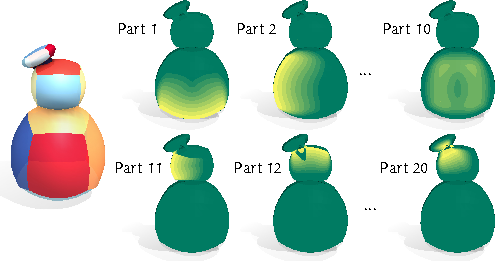
\includegraphics[width=3.33in]{figures/distance_weight_puft.pdf}
%   \caption{Our distance weights decay smoothly from 1.0 (yellow) to 0.0 (green) when moving away from its closest surface. Here we visualize the distribution of the distance weights (with cutoff distance 5.0) corresponding to each part.   
%   }
%   \label{fig:distance_weight_puft}
%   \vspace{-5pt}
% \end{figure} 
% %
% %
% \begin{figure}
%   \centering
%   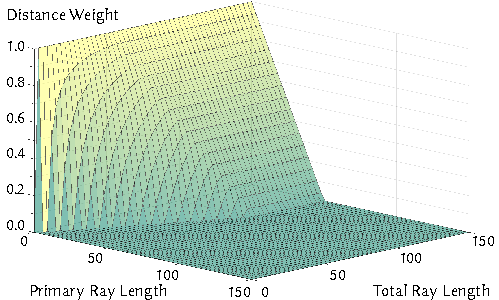
\includegraphics[width=3.33in]{figures/plot_distance_weight.pdf}
%   \caption{We plot the distance weight with respect to the primary and total ray length. Here the cutoff distance is 50.
%   }
%   \label{fig:plot_distance_weight}
%   \vspace{-5pt}
% \end{figure} 

%kinematic model is expressive
% \begin{figure}
%   \includegraphics[width=\columnwidth]{example-image-a}
%   \caption{Take an intesting geometry (maybe that geometry processing cacture), deform it, do our shape matching and then reconstruct the deformed pose. Do this for a bunch of poses (show's kinematic model is good).}
%   \label{fig:deform}
% \end{figure}

%% Results that relate to simulation output
%correctness
\begin{figure}[h]
  \includegraphics[width=\columnwidth]{figures/patch_test.pdf}
  \caption{2D patch test. By applying affine transformations to the boundary of the original undeformed model (left), we show that solving the static problem gives rigid motion for rotation and constant strain for shearing and stretching (right).}
  % \caption{2D patch test. Left: the original undeformed model defined by four surface elements on the boundary. Right:  applying affine transformations to the boundary and show that solving the static problem gives rigid motion for rotation and constant strain for shearing and stretching}
  \label{fig:patchtest}
\end{figure}


We first validate the physical plausibility of our method using a small 2D patch test~(\reffig{patchtest}). 
Here the test object is a square made of four edges (not joined at the corners) simulated using linear polynomials with a single deformation center.
We apply a battery of boundary conditions and resolve the deformation of the element by minimizing the elastic potential.
We note that SEM is able to represent rigid motions, as well as shearing and anisotropic stretching. 
This implies that, with sparse weights, SEM can resolve these motions locally, leading to physically plausible simulation results.

We further demonstrate \emph{qualitative} convergence of SEM with respect to linear tetrahedral finite elements when increasing the number of patches in use.
In \reffig{convergence}, we compare identical cantilevered beams, simulated using a Neohookean constitutive model (Young's Modulus $=$ $0.001$ GPa, Poisson's Ratio $=$ $0.45$) and implicit time integration with a timestep of $0.01$s. 
We use SEM with quadratic polynomials for this test and observe that our SEM simulation, made of 24 independent NURBS patches, shows good agreement with FEM. Each subdivision of the NURBS beam enables more complicated kinematics, 
but very few surface elements are needed to produce compelling results.

\begin{figure}[h]
  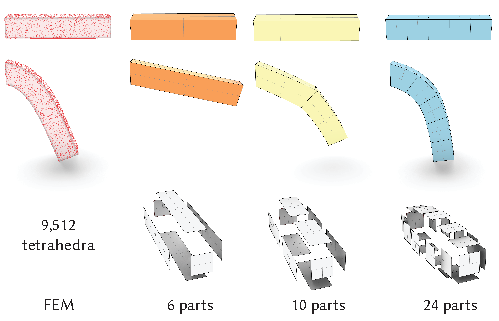
\includegraphics[width=\columnwidth]{figures/beams.pdf}
  \caption{Our SEM simulation is able to qualitatively converge to a high resolution FEM simulation result (left) as we increase the number of surfaces in the model (right). }
  \label{fig:convergence}
\end{figure}

We also show that our raycasting weight computation is able to create shape-aware output. \reffig{independence} shows that manipulating
parts that are nearby but separated will behave in an appropriately independent fashion. Our grumpy model is capable of extending 
its leg without causing unrealistic deformations in the plant foot.

\begin{figure}[h]
  \includegraphics[width=\columnwidth]{figures/independent_movement}
  \caption{Our raycasting weight computation produces share-aware blending weights. Here the locality of our blending weights allows the two legs of the grumpy model to move independently. }
  \label{fig:independence}
\end{figure}

% relaxed modelling constraints
By virtue of its meshless nature, SEM is robust to a wide range of challenging models with large gaps and disconnected primitives.
\reffig{fig:chicken} shows frames from a simulation of a rubber chicken. Note that the chicken model itself features large gaps between the individual NURBS parts. 
Despite the lack of explicit connectivity, the SEM blending weights have the effect of implicitly enforcing connectivity at these seams. 

\begin{figure*}[htp]
  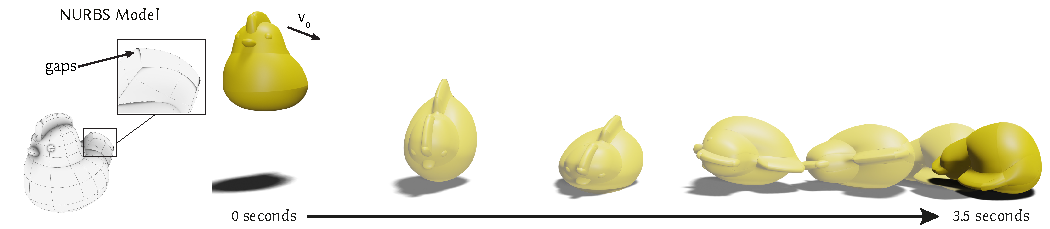
\includegraphics[width=\textwidth]{figures/chicken.pdf}
  \caption{Simulation of a chicken model with gaps between surfaces.}
  \label{fig:chicken}
\end{figure*}

SEM is also robust to intersections in modelling input. \reffig{badmodels} shows simulations of two jelly coffee mugs. 
The top row shows a model with negligible overlap, whereas the bottom row shows the result of a careless modeller who has deeply embedded the handle of the mug in the body in order to attach it, creating a large area of overlap.
In both cases SEM produces a plausible physically-based animation without requiring additional model clean-up.

\begin{figure}[H]
  \includegraphics[width=\columnwidth]{figures/mug_overlap}
  \caption{Our SEM is robust to overlapping regions and self-intersections. Here the simulation result of the coffee mug with overlapping handle (bottom) still matches its corresponding counterpart without negligible overlaps (top). }
  % \caption{Coffee mug with overlapping handle. (top) row of models with increasing overlap (middle) single weight image showing behaviour in the overlapping region, (bottom) simulation result for each one}
  \label{fig:badmodels}
\end{figure}

%different material parameters / material models 
Since the equations of motion for SEM are derived using a general elastic potential, it is theoretically capable of supporting arbitrary elastic constitutive models.
% We derive the equations of motion for SEM using a general elastic potential and thus SEM supports arbitrary constitutive models. 
\reffig{rocket} shows a rocket ship simulated with both high stiffness (steel) and low stiffness materials (rubber). 
In both cases intuitive and visually pleasing results are created wherein the trajectories correctly reflect the desired material characteristics.  
%multiple materials
\begin{figure*}[htp]
  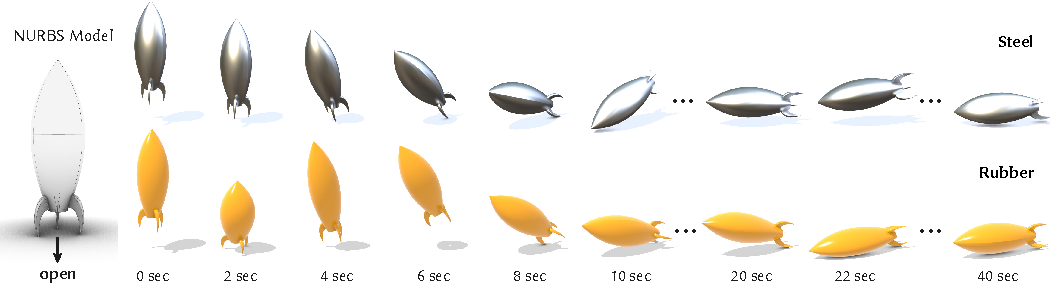
\includegraphics[width=\textwidth]{figures/rocket.pdf}
  \caption{SEM is able to produce animation using a wide variety of material parameters. Here we simulate both a steel and rubber rocket ship. 
  To make this even more challenging, the rocket model is an open surface (at the bottom), but a plausible animation is still generated.}
  \label{fig:rocket}
\end{figure*}

SEM also supports the simulation of objects made up of heterogenous materials. By specifying different material properties inside nested 
parts we are able to simulate a drag racing wheel with a metal hub and soft rubber tread~(\reffig{tire}).

\begin{figure}[h]
  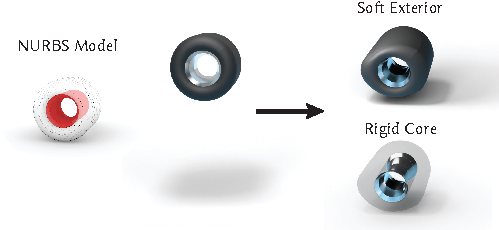
\includegraphics[width=\columnwidth]{figures/tire}
  \caption{Our SEM is directly applicable to the simulation of objects with heterogenous materials.}
  \label{fig:tire}
\end{figure}


% %different surface reps
% Though we focus on NURBS surface representations, the only NURBS specific construction in the SEM method is the Jacobian \refeq{velocity_jacobian}.
% Many other boundary representations admit a linear representation and are thus directly consumable by our method.
% \reffig{subd} shows an example of applying our SEM method to a subdivision model by making such a modification.
% \begin{figure}[h]
%   \includegraphics[width=\columnwidth]{example-image-a}
%   \caption{show subd simulation if we have it. If it works really well we'll just mix subds and nurbs throughout the paper. }
%   \label{fig:subd}
% \end{figure}

% different time integration scheme
\nicetohave{Integration Figure}
%\begin{figure}[h]
%  \includegraphics[width=\columnwidth]{example-image-a}
%  \caption{show mug simulation using newton's method, linearly implicit Euler \Honglin{Maybe I can do that quickly}. }
%  \label{fig:time_integration}
%\end{figure}

%editing example
For downstream applications, the output of  SEM simulation is itself editable in a NURBS modelling program (see \reffig{edit}). 
This can be useful for visual effects pipelines, allowing artists to easily post process animations using the same tools in which they were created.
\begin{figure}[h]
  \includegraphics[width=\columnwidth]{example-image-a}
  \caption{Here we show the output of an SEM animation loaded into Rhinoceros 3D 7 for additional editing.}
  \label{fig:edit}
\end{figure}

%show stoppers
Finally we show a few additional examples, highlighting the ability of SEM to handle complex simulations involving deformation, contact and friction.
In \reffig{staypuft} we show two astronauts in jaunty space suits collide in zero gravity while in \reffig{starship} 
we show an animation of the Space-V starship landing on Mars in a graceful way.

\begin{figure*}[htp]
  \includegraphics[width=\textwidth,height=3in]{example-image-a}
  \caption{Two astronauts, in jaunty spacesuits collide while spacewalking in zero-g.}
  \label{fig:staypuft}
\end{figure*}

\begin{figure*}[htp]
  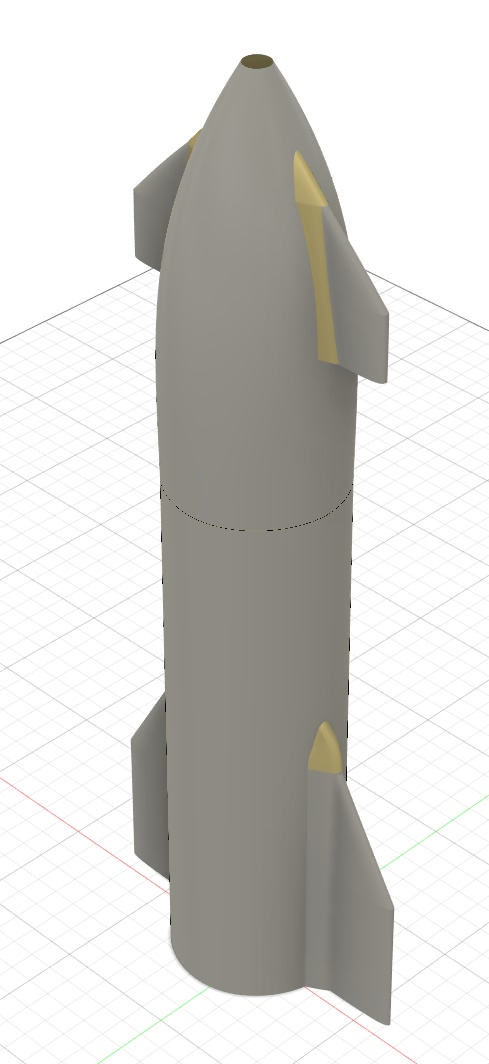
\includegraphics[width=\textwidth,height=3in]{figures/starship.pdf}
  \caption{The Space-V starship makes a graceful landing on the red planet. }
  \label{fig:starship}
\end{figure*}

\section{Future Work and Conclusions}
\dave{mention that constraint from complimentary dynamics could be used to replace error energy}
We have presented the Shape Matching Element Method (SEM), the first completely meshless approach to direct simulation of NURBS models.
Our approach is unique in its ability to infer volumetric shape from surface only models,
including ones with intersecting geometry, between parts and other defects common to non-engineering models.
Our method allows simulation of such input directly, with a variety of contitutive models and time integration schemes
and is compatibale with standard methods for collision resolution. 
We believe that SEM is a signficant improvement over standard physics-based animtion pipelines for NURBS models. 
As evidence of the efficacy of our approach, the authors submit that many of the examples in this paper were constructed ourselves
(since the standard graphics menagerie is not available as NURBS models). 
Modelling, cleaning, meshing and simulating would've been a burdensome experience without SEM's
ability to leap directly from (often hastily) constructed models to physics-based animations.

But SEM as it's presented here is only the beginning and we believe there are many exciting areas of future work to explore.
We are very excited to couple SEM to machine learning approaches for design, parameter estimation and Real2Sim applications.
One of the cumbersome elements in using finite element simulation for such problems is the need for robust, differentiable volumetric meshing.
While there has been some work on this~\dave{cite} it is far from a solved problem.
SEM removes this bottleneck entirely, providing a direct mapping from geometric input to physics-driven output. 
We believe this will both enable simpler and more robust algorithms for  physics-based ML and 
allow the application of such algorithms to a much broader class of problems. 

SEM itself has much room for addition.
First, while we focus on NURBS surfaces here, the only part of SEM that is NURBS specific is the shape matching operation.
We believe there is potential to allow mixed models (models which include polygonal meshes, particles, subdivision surfaces and NURBS)
by extending the range of shape matching operations used by the algorithm. The shape matching operation itself could be improved to be material aware 
(to better handle heterogenous materials) or to be robust to noisy data (allowing direct simulation of scanned data). The Finite Element method took over 
40 years to take over the world of simulation. 
We see this work as the first step in a similar journey for SEM

To encourage future research on SEM the authors will release our SEM implementation under a permissive license as well as all models created for this submission.


%%
%% The next two lines define the bibliography style to be used, and
%% the bibliography file.
\bibliographystyle{ACM-Reference-Format}
\bibliography{references}

Dump of some equations
\begin{align*}
    \mathbf{M(X)} = (X_0 - \bar{X}_0, X_1 - \bar{X}_1)\\
    \bar{\mathbf{x}} = \frac{1}{n}\sum_i^n x_i \\
    \bar{\mathbf{X}} = \frac{1}{n}\sum_i^n X_i \\
\end{align*}




\end{document}
